\documentclass[journal]{IEEEtran}

\usepackage{url}
\usepackage{amsmath,amssymb}

\hyphenation{op-tical net-works semi-conduc-tor}

\usepackage{graphicx}


\begin{document}

\title{LQ-ICIF: Learnable Query-Guided Image-Comment Interaction Fusion for Image Aesthetic Assessment}

\author{First A. Author, \IEEEmembership{Fellow, IEEE}, Second B. Author, and Third C. Author, Jr., \IEEEmembership{Member, IEEE}
\thanks{This paragraph of the first footnote will contain the date on which you submitted your paper for review. It will also contain support information, including sponsor and financial support acknowledgment. For example, ``This work was supported in part by the U.S. Department of Commerce under Grant 123456.''}
\thanks{The next few paragraphs should contain the authors' current affiliations, including current address and e-mail. For example, First A. Author is with the National Institute of Standards and Technology, Boulder, CO 80305 USA (e-mail: author@boulder.nist.gov).}
\thanks{Second B. Author, Jr., was with Rice University, Houston, TX 77005 USA. He is now with the Department of Physics, Colorado State University, Fort Collins, CO 80523 USA (e-mail: author@lamar.colostate.edu).}}

\markboth{Journal of \LaTeX\ Class Files, Vol. 14, No. 8, August 2015}
{Shell \MakeLowercase{\textit{et al.}}: Bare Demo of IEEEtran.cls for IEEE Journals}
\maketitle

\begin{abstract}
Image Aesthetic Assessment (IAA) has attracted wide interest in recent years, but it remains challenging due to its highly subjective and ambiguous nature. With the prevalence of social media, user comments can provide rich aesthetics-aware semantic information and human observers typically evaluate images from the perspective of aesthetic attributes. Motivated by the effectiveness of learnable queries in extracting task-specific features from frozen models, we propose LQ-ICIF (Learnable Queries with Intra-Cross Interaction Fusion), a multimodal framework that applies learnable query-guided intra-cross interaction hierarchically across encoder layers, with multi-layer outputs aggregated via a global token and further refined by aesthetic attribute priors. Experiments on AVA-Comments demonstrate that LQ-ICIF achieves state-of-the-art performance on multimodal IAA, with an SRCC of 0.915 and a PLCC of 0.920.
\end{abstract}
\begin{IEEEkeywords}
Image aesthetic assessment, learnable queries, multimodal fusion, hierarchical interaction, aesthetic attributes.
\end{IEEEkeywords}

\IEEEpeerreviewmaketitle

\section{Introduction}

\IEEEPARstart{I}{mage} aesthetic assessment (IAA) aims to automatically predict human aesthetic perception of images. Owing to its wide applications in fields such as image retrieval, photo recommendation, automatic enhancement, and social media content management, this task has attracted growing interest in recent years.

\begin{figure}[!t]
\centering
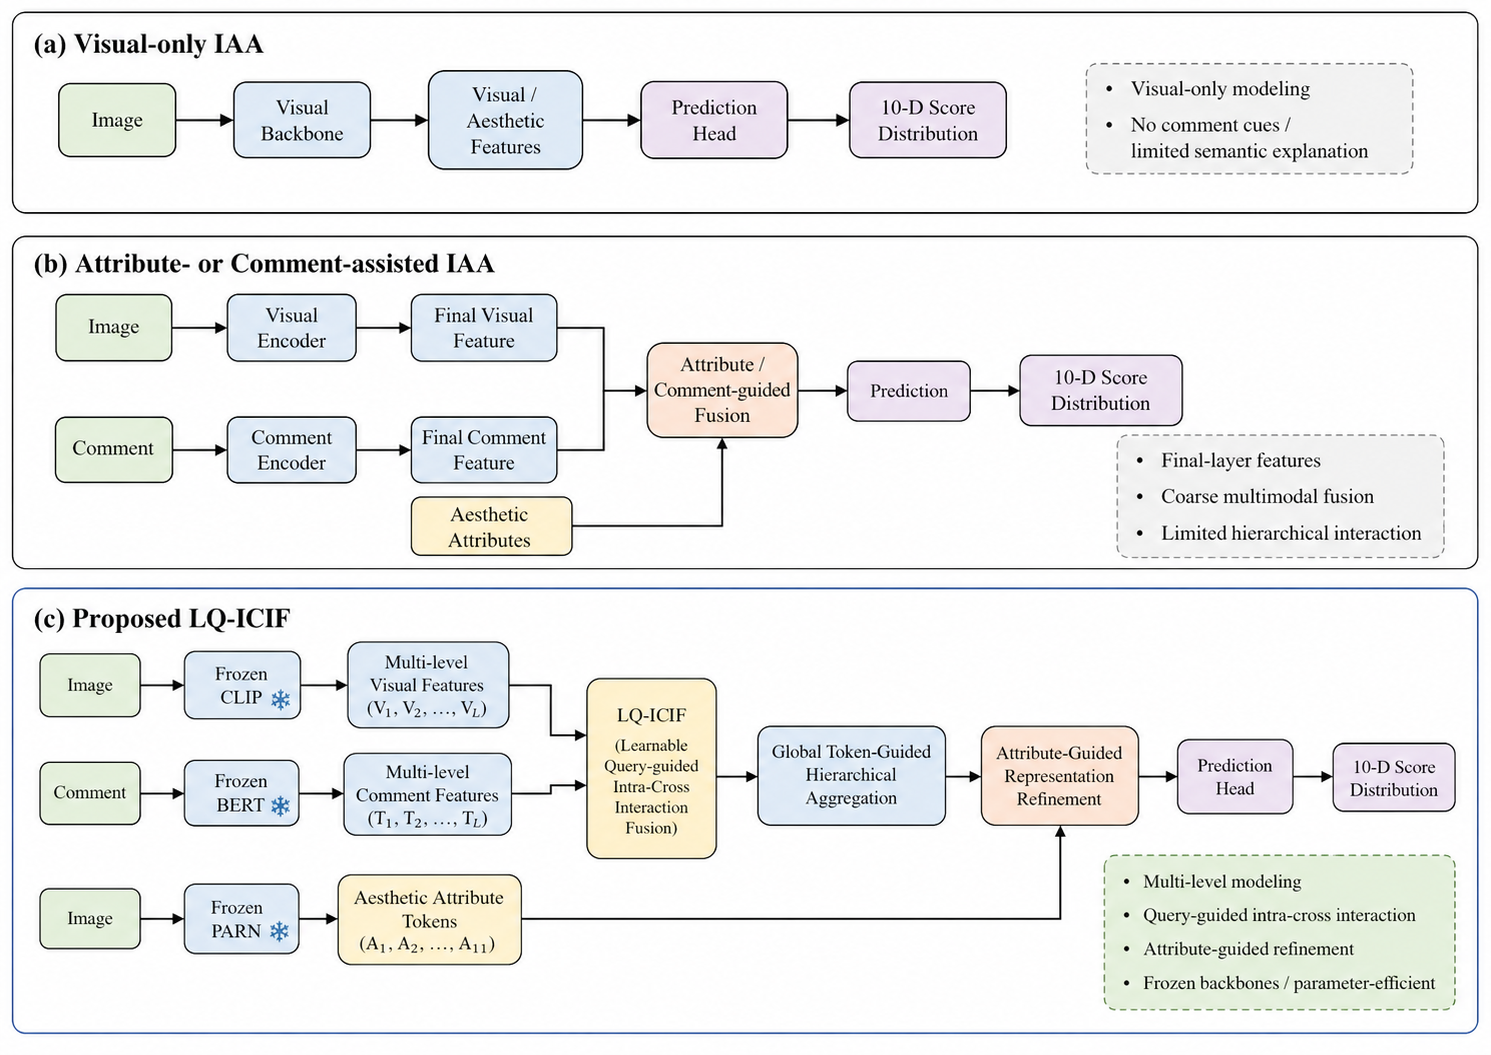
\includegraphics[width=\columnwidth]{method_comparison.png}
\caption{Comparison of representative image aesthetic assessment paradigms. Unlike visual-only and coarse auxiliary-fusion methods, LQ-ICIF exploits multi-level image-comment interaction and attribute-guided refinement for aesthetic score distribution prediction.}
\label{fig:method_comparison}
\end{figure}

Due to its highly abstract nature, IAA remains a challenging research topic. Early IAA approaches focused on designing hand-crafted features based on photographic rules. More recently, with the prevalence of deep learning, distribution prediction methods, such as NIMA, utilize Earth Mover's Distance (EMD) to predict aesthetic score distributions. However, relying solely on aesthetic score labels provides limited supervision information, which may result in a neglect of details.

Based on existing works, user comments can not only provide complementary semantic features, but also describe attribute characteristics. In recent years, several methods employ aesthetic attributes to connect visual and textual representations. These studies indicate that it is of great value to jointly model visual appearances, textual feedback, and aesthetic attributes.

Recently, large-scale pre-trained models have demonstrated strong capabilities. Learnable queries have also been shown to be effective in extracting useful task-specific features from frozen pre-trained backbones. Therefore, we propose LQ-ICIF, which leverages learnable queries to extract aesthetics-related features from frozen visual and textual encoders for images and user comments, and further achieves more effective multi-modal aesthetic representations via image-comment interaction and aesthetic attribute-guided refinement.

Specifically, LQ-ICIF freezes pre-trained encoders including CLIP, BERT, and an attribute encoder, and only trains lightweight fusion and prediction modules. The framework first employs learnable queries to extract modality-specific aesthetic features from images and comments, and then models the complementary relationships between images and comments via cross-modal attention. Subsequently, a global token is utilized to aggregate multi-layer features, and the aesthetic attribute priors extracted by the attribute encoder are introduced to refine the final representation, thereby predicting the aesthetic score distribution.

The primary contributions of this paper are summarized as follows:
\begin{itemize}
\item We propose a multi-modal framework for aesthetic score distribution prediction. By freezing the pre-trained visual, textual, and attribute encoders, this framework integrates image, comment, and aesthetic attribute information via lightweight modules.
\item We propose the LQ-ICIF module, a learnable query-guided image-comment interaction mechanism, which utilizes learnable queries to extract aesthetics information from frozen visual and textual features and models the complementary relationship between image contents and user comments via cross-modal attention.
\item We design a global token aggregation module and an attribute-guided refinement module to integrate multi-level aesthetic features and introduce structured aesthetic attribute priors, respectively, thereby enhancing the prediction performance.
\end{itemize}

\section{Method}

\subsection{Problem Formulation}

Given the $i$-th image and its corresponding user comment $(I_i,C_i)$, this paper aims to learn a mapping function $f(\cdot)$ to predict the discrete aesthetic score distribution:
\begin{equation}
\hat{\mathbf{y}}_i=f(I_i,C_i),
\end{equation}
where $\hat{\mathbf{y}}_i\in\mathbb{R}^{K}$ denotes the predicted aesthetic score distribution, and $K$ represents the number of aesthetic scores, or score levels. For the public AVA dataset, $K=10$. The ground-truth score distribution $\mathbf{y}_i$ satisfies:
\begin{equation}
\sum_{k=1}^{K}y_i^k=1.
\end{equation}
Based on the predicted score distribution, the mean aesthetic score $\mu_i$ of the image can be further calculated as:
\begin{equation}
\label{eq:mean_score}
\mu_i=\sum_{k=1}^{K}k\cdot\hat{y}_i^k.
\end{equation}

Currently, learning the aesthetic score distribution from an image and its associated user comments still encounters several challenges. On the one hand, image aesthetics is intrinsically highly abstract and subjective, leading to the lack of a stable mapping between visual features and aesthetic score distributions. On the other hand, although user comments provide rich information from diverse perspectives, they often lack semantic completeness. Therefore, how to effectively fuse the complementary information from both visual and textual modalities is the key to achieving accurate aesthetic score distribution prediction.

To alleviate the aforementioned issues, we introduce aesthetic attributes as auxiliary information. Previous studies have demonstrated that people often comment on images from the perspective of attributes. Consequently, aesthetic attributes can serve as a semantic bridge between the visual and textual modalities, helping the model capture aesthetic features. To this end, multi-modal feature extraction is performed on the input image and its comment, which is formalized as follows.

For the input image $I_i$ and its comment $C_i$, CLIP and BERT are employed as the visual encoder $E_v(\cdot)$ and textual encoder $E_t(\cdot)$, respectively, to extract their hidden state features from multiple layers:
\begin{equation}
\{\mathbf{V}_i^l\}_{l=1}^{L}=E_v(I_i), \quad
\{\mathbf{T}_i^l\}_{l=1}^{L}=E_t(C_i),
\end{equation}
where $\mathbf{V}_i^l\in\mathbb{R}^{N_v\times H_v}$ denotes the visual token features at the $l$-th layer, $N_v$ is the number of visual tokens, and $H_v$ represents the visual feature dimension; $\mathbf{T}_i^l\in\mathbb{R}^{N_w\times H_t}$ denotes the textual token features at the $l$-th layer, $N_w$ is the maximum comment length, and $H_t$ represents the textual feature dimension; $L$ is the number of selected feature layers. The parameters of both encoders remain frozen. Concurrently, a pre-trained attribute encoder $E_a(\cdot)$ is used to extract the aesthetic attribute features from the image:
\begin{equation}
\mathbf{A}_i=E_a(I_i),
\end{equation}
where $\mathbf{A}_i\in\mathbb{R}^{M}$ represents the extracted global attribute features, and $M$ is the feature dimension. Since these features are extracted from different pre-trained backbones, their feature dimensions vary. Therefore, projection layers are further utilized to map them into a unified feature space:
\begin{equation}
\tilde{\mathbf{V}}_i^l=P_v(\mathbf{V}_i^l), \quad
\tilde{\mathbf{T}}_i^l=P_t(\mathbf{T}_i^l), \quad
\tilde{\mathbf{A}}_i=P_a(\mathbf{A}_i),
\end{equation}
where $P_v(\cdot)$, $P_t(\cdot)$, and $P_a(\cdot)$ represent the projection layers for the visual, textual, and attribute features, respectively. Each projection layer consists of a linear transformation and a layer normalization layer. After projection, we obtain $\tilde{\mathbf{V}}_i^l\in\mathbb{R}^{N_v\times d}$, $\tilde{\mathbf{T}}_i^l\in\mathbb{R}^{N_w\times d}$, and $\tilde{\mathbf{A}}_i\in\mathbb{R}^{d}$, where $d$ denotes the unified feature dimension. Through this unified representation, aesthetic information from different modalities and different layers can interact and fuse within the same feature space.

\begin{figure*}[!t]
\centering
\includegraphics[width=\textwidth]{lq_icif_overview.png}
\caption{Framework of the proposed LQ-ICIF. It integrates (1) learnable query-guided intra-cross interaction fusion, modeling hierarchical image-comment relations with lightweight trainable queries; (2) global token-guided hierarchical aggregation, summarizing multi-level visual and textual features into a compact multimodal representation; and (3) attribute-guided representation refinement, injecting PARN-based aesthetic attribute priors before distribution prediction.}
\label{fig:lqicif_overview}
\end{figure*}

As illustrated in Fig.~\ref{fig:lqicif_overview}, the proposed method models multi-modal aesthetic features in three stages. First, learnable queries are employed to extract intra-modal aesthetic representations from visual and textual features, respectively, and further model the cross-modal interactions between images and comments. Subsequently, a hierarchical aggregation module is used to summarize the multi-layer visual and textual features, obtaining a discriminative multi-modal aesthetic representation. Finally, an aesthetic attribute-guided calibration module is introduced to incorporate attribute information into the multi-modal representations, refining the fused features to enhance the accuracy of aesthetic score distribution prediction.

\subsection{Learnable Query-Guided Intra-Cross Interaction Fusion}

Rather than applying cross-attention to all visual and textual tokens at once, we use learnable queries to obtain compact aesthetic features before cross-modal exchange. For the $l$-th visual-textual feature pair $(\tilde{\mathbf{V}}_i^l,\tilde{\mathbf{T}}_i^l)$, two query sets, $\mathbf{Q}_{l,0}^{V}$ and $\mathbf{Q}_{l,0}^{T}$, first attend to their own modality:
\begin{equation}
\begin{aligned}
\mathbf{Q}_{l}^{V}
&=\mathrm{Attn}(\mathbf{Q}_{l,0}^{V},\tilde{\mathbf{V}}_i^l,\tilde{\mathbf{V}}_i^l),\\
\mathbf{Q}_{l}^{T}
&=\mathrm{Attn}(\mathbf{Q}_{l,0}^{T},\tilde{\mathbf{T}}_i^l,\tilde{\mathbf{T}}_i^l).
\end{aligned}
\end{equation}
The intra-modal step keeps modality-specific aesthetic features, such as visual composition or subjective textual impressions. Then, cross-modal attention exchanges complementary image-comment features without directly merging all tokens:
\begin{equation}
\begin{aligned}
\hat{\mathbf{Q}}_{l}^{V}
&=\mathrm{Attn}(\mathbf{Q}_{l}^{V},\tilde{\mathbf{T}}_i^l,\tilde{\mathbf{T}}_i^l),\\
\hat{\mathbf{Q}}_{l}^{T}
&=\mathrm{Attn}(\mathbf{Q}_{l}^{T},\tilde{\mathbf{V}}_i^l,\tilde{\mathbf{V}}_i^l).
\end{aligned}
\end{equation}
The resulting cross-attended queries are added back to the intra-modal queries to obtain $\mathbf{F}_{l}^{V}$ and $\mathbf{F}_{l}^{T}$. Applying this block to multiple layers captures hierarchical image-comment interactions while keeping the pretrained encoders frozen.

\subsection{Global Token-Guided Hierarchical Aggregation}

Different feature levels capture different aesthetic features, from color and texture to composition, semantics, and subjective impressions, so simply using the final layer may discard useful features. We first mean-pool $\mathbf{F}_{l}^{V}$ and $\mathbf{F}_{l}^{T}$ into layer descriptors $\mathbf{z}_{l}^{V}$ and $\mathbf{z}_{l}^{T}$. The descriptors are then concatenated with learnable global tokens and processed by self-attention:
\begin{equation}
\begin{aligned}
\mathbf{S}^{V}
&=\mathrm{SA}([\mathbf{g}_{0}^{V};\mathbf{z}_{1}^{V};\ldots;\mathbf{z}_{L}^{V}]),\\
\mathbf{S}^{T}
&=\mathrm{SA}([\mathbf{g}_{0}^{T};\mathbf{z}_{1}^{T};\ldots;\mathbf{z}_{L}^{T}]).
\end{aligned}
\end{equation}
The updated global tokens serve as modality-level summaries:
\begin{equation}
\mathbf{F}_{\mathrm{cat}}=[\mathbf{h}^{V};\mathbf{h}^{T}], \quad
\mathbf{h}^{V}=\mathbf{S}^{V}_{0},\ \mathbf{h}^{T}=\mathbf{S}^{T}_{0}.
\end{equation}
Thus, the model adaptively selects useful features from multiple feature levels and forms a compact multimodal representation for refinement.

\subsection{Attribute-Guided Representation Refinement}

Although comments provide useful subjective features, they may not consistently cover photographic properties that influence aesthetic judgment. To make the final representation less dependent on implicit image-comment fusion, the frozen PARN branch provides structured aesthetic priors. Given $I_i$, PARN produces a global attribute feature $\mathbf{g}_i$ and attribute scores $\mathbf{s}_i=[s_i^1,\ldots,s_i^A]$, covering explicit photographic properties. Each score is combined with $\mathbf{g}_i$ and projected into an attribute token:
\begin{equation}
\mathbf{a}_i^j=P_r([\mathbf{g}_i;s_i^j]), \quad j=1,\ldots,A.
\end{equation}
The attribute tokens form $\mathbf{A}_i=[\mathbf{a}_i^1,\ldots,\mathbf{a}_i^A]$, which refine the aggregated multimodal representation by cross-attention:
\begin{equation}
\hat{\mathbf{F}}_i=\mathrm{CrossAttn}(\mathbf{F}_{\mathrm{cat}},\mathbf{A}_i,\mathbf{A}_i).
\end{equation}
In this way, the final representation is guided toward perceptually meaningful aesthetic dimensions before prediction, rather than relying only on implicit multimodal fusion.

\subsection{Aesthetic Score Distribution Prediction}

The refined representation $\hat{\mathbf{F}}_i$ is fed into an MLP head followed by softmax to estimate the full rating distribution:
\begin{equation}
\hat{\mathbf{y}}_i=\mathrm{Softmax}(\mathrm{MLP}(\hat{\mathbf{F}}_i)),
\end{equation}
The softmax output keeps the full uncertainty of human ratings instead of collapsing them into a single scalar during training. Following distribution-based IAA methods, the normalized ground-truth rating histogram $\mathbf{y}_i$ supervises $\hat{\mathbf{y}}_i$ with the Earth Mover's Distance (EMD):
\begin{equation}
\mathcal{L}_{\mathrm{emd}} =
\left(
\frac{1}{K}\sum_{k=1}^{K}
\left|
\mathrm{CDF}_{\hat{\mathbf{y}}_i}(k)-
\mathrm{CDF}_{\mathbf{y}_i}(k)
\right|^r
\right)^{1/r},
\end{equation}
where $\mathrm{CDF}_{\hat{\mathbf{y}}_i}(k)=\sum_{j=1}^{k}\hat{y}_i^j$, $\mathrm{CDF}_{\mathbf{y}_i}(k)=\sum_{j=1}^{k}y_i^j$, and $r=2$. The final mean score is computed by \eqref{eq:mean_score}.

\section{Experiments}
\label{sec:experiments}

\subsection{Experimental Protocols}

We conduct experiments on AVA [2], which contains 222,383 training, 11,707 validation, and 19,805 test images in our split, each with a 10-bin rating histogram. We further use AVA-Comments, which provides 3,602,206 comments for 255,530 images.

We report SRCC, PLCC, ACC, and EMD to evaluate ranking consistency, linear correlation, binary classification, and distribution prediction. The AVA rating histogram is directly normalized as ground truth. All experiments are implemented in PyTorch on a single NVIDIA GeForce RTX 5060 Ti GPU.

\subsection{Implementation Details}

All comments matched to an image are concatenated as text input, while missing comments are replaced by a ``no comment'' token. Images are resized to $224\times224$ with random horizontal flipping during training. We freeze CLIP ViT-L/14, BERT-base, and PARN, and train only the lightweight modules for 10 epochs using AdamW with learning rate $1\times10^{-4}$, batch size 16, and a loss combining EMD, mean-score MSE, and pairwise ranking terms.

\begin{table}[!t]
\caption{Performance Comparison on Aesthetic Assessment Datasets}
\label{tab:main_comparison}
\centering
\scriptsize
\setlength{\tabcolsep}{1.6pt}
\begin{tabular}{c|c|l|cccc}
\hline
Category & Input$^{1}$ & Method & \multicolumn{4}{c}{AVA$^{2}$} \\
\cline{4-7}
 & & & SRCC & PLCC & Acc. & EMD \\
\hline
Visual & $I$ & NIMA [3] & 0.612 & 0.636 & 81.51 & 0.050 \\
& $I$ & GPF-CNN [23] & 0.690 & 0.704 & 81.81 & 0.045 \\
& $I$ & HLA-GCN [16] & 0.665 & 0.687 & 84.60 & 0.043 \\
& $I$ & MUSIQ [17] & 0.726 & 0.738 & 81.50 & -- \\
& $I$ & TANet [18] & 0.758 & 0.765 & -- & 0.047 \\
& $I$ & MILNet [21] & 0.758 & 0.758 & 81.80 & -- \\
& $I$ & IAA-LQ [19] & 0.791 & 0.790 & -- & -- \\
& $I$ & TCD-G [22] & 0.817 & 0.818 & 84.20 & -- \\
& $I$ & AesMamba-V$\dagger$ [20] & 0.769 & 0.774 & 85.00 & -- \\
\hline
Multi. & $I+C$ & VILA-R [5] & 0.774 & 0.774 & -- & -- \\
& $I+C+A$ & AAM-Net [8] & 0.780 & 0.803 & 85.69 & 0.037 \\
& $I+C+A$ & AMM-Net [7] & 0.816 & 0.830 & 87.58 & 0.035 \\
& $I+C$ & MMLQ [6] & 0.876 & 0.896 & 89.03 & 0.029 \\
& $I+C$ & MSCAN$^{\ddagger}$ [24] & 0.852 & 0.862 & 86.70 & 0.035 \\
& $I+C$ & AesMamba-M$^{\ddagger}$ [20] & 0.892 & 0.899 & 89.60 & 0.031 \\
& $I+C+A$ & Ours & \textbf{0.9147} & \textbf{0.9201} & 87.40 & 0.0410 \\
\hline
\end{tabular}
\vspace{2pt}
\begin{flushleft}
\scriptsize
$^{1}$ $I$, $C$, and $A$ denote image, comment, and attribute prior.\\
$^{2}$ Results are from original papers; ``--'' denotes unreported metrics. Bold marks the best SRCC/PLCC among listed methods.\\
$\dagger$ denotes the stronger AesMamba visual variant. $\ddagger$ denotes AVA-Captions~[13] results.
\end{flushleft}
\end{table}

\subsection{Performance Comparison}

Table~\ref{tab:main_comparison} compares LQ-ICIF with visual-only and multimodal IAA methods on AVA. LQ-ICIF obtains the highest rank and linear correlations among the listed methods, reaching 0.9147 SRCC and 0.9201 PLCC while keeping CLIP, BERT, and PARN frozen. Its accuracy and EMD remain competitive, and the correlation gains indicate that the lightweight image-comment interaction and refinement modules are effective for aesthetic score distribution prediction.

\subsection{Ablation Study}

Table~\ref{tab:ablation} reports ablation results from single-modality baselines to the full LQ-ICIF model.

\begin{table}[!t]
\caption{Ablation Study of LQ-ICIF on AVA}
\label{tab:ablation}
\centering
\scriptsize
\setlength{\tabcolsep}{1.4pt}
\begin{tabular}{l|c|cccc|cccc}
\hline
Method & Input & Cat. & DCA & ICIF & Full & SRCC & PLCC & ACC & EMD \\
\hline
$A_0$ & $I$     & -- & -- & -- & -- & 0.7570 & 0.7582 & 81.46 & 0.0614 \\
$A_1$ & $C$     & -- & -- & -- & -- & 0.8193 & 0.8339 & 82.21 & 0.0539 \\
$A_2$ & $I+C$   & \checkmark & -- & -- & -- & 0.8836 & 0.8912 & 85.87 & 0.0455 \\
$A_3$ & $I+C$   & -- & \checkmark & -- & -- & 0.9120 & 0.9182 & 86.94 & 0.0409 \\
$A_4$ & $I+C$   & -- & -- & \checkmark & -- & 0.9145 & \textbf{0.9204} & 87.10 & \textbf{0.0407} \\
$A_5$ & $I+C+A$ & -- & -- & \checkmark & \checkmark & \textbf{0.9147} & 0.9201 & \textbf{87.40} & 0.0410 \\
\hline
\end{tabular}
\vspace{2pt}
\begin{flushleft}
\scriptsize Cat.: final-layer CLIP/BERT concatenation. DCA: direct single-layer cross-attention following MMLQ~[6]. ICIF: query-guided intra-cross interaction fusion. Full: complete LQ-ICIF with hierarchical aggregation and attribute-guided refinement. Best values are bolded, and lower EMD is better.
\end{flushleft}
\end{table}

The first three variants show the value of multimodal modeling. Compared with visual-only and text-only baselines, simple image-comment concatenation improves SRCC to 0.8836 and reduces EMD to 0.0455, indicating that comments provide useful complementary features. Replacing this coarse fusion with direct cross-attention further raises SRCC to 0.9120, confirming the importance of explicit image-comment interaction.

The comparison between $A_3$ and $A_4$ verifies the proposed ICIF design. By preserving modality-specific features before cross-modal exchange, ICIF improves SRCC/PLCC to 0.9145/0.9204. The full model ($A_5$) remains in the same high-performance range and achieves the best SRCC, indicating that ICIF is the main source of improvement while hierarchical aggregation and attribute refinement serve as compact final design components.

It is also worth noting that the full model does not improve every metric monotonically over $A_4$. This suggests that the main performance gain comes from robust image-comment feature interaction, while the additional aggregation and attribute refinement mainly stabilize the final representation with multi-level and structured photographic features.

\subsection{Model Complexity Analysis}

Table~\ref{tab:complexity} compares trainable parameters, adaptation GMACs, and AVA performance. GMACs are measured with \texttt{thop} on a $224\times224$ image and the corresponding text input when applicable. For frozen-encoder methods, backbone computations are excluded to focus on task-specific modules.

\begin{table}[!t]
\caption{Comparison of Model Complexity and Performance}
\label{tab:complexity}
\centering
\footnotesize
\setlength{\tabcolsep}{3.2pt}
\begin{tabular}{l|l|ccc}
\hline
Method & Input & Train.\,Params\,(M) & GMACs & SRCC \\
\hline
TANet [18] & $I$ & 13.883 & 2.165 & 0.758 \\
Charm [25] & $I$ & 22.064 & 5.525 & -- \\
AesMamba-V [20] & $I$ & 22.818 & 2.843$^{*}$ & 0.769 \\
MMLQ [6] & $I+C$ & 60.266 & 6.193 & 0.876 \\
AesMamba-M [20] & $I+C$ & 139.388 & 3.539$^{*}$ & 0.892 \\
Ours & $I+C+A$ & 175.870 & 10.837 & \textbf{0.9147} \\
\hline
\end{tabular}
\vspace{2pt}
\begin{flushleft}
\scriptsize $^{*}$ GMACs are approximate because the custom \texttt{mamba\_ssm} CUDA operator was unavailable; parameter counts are unaffected. ``--'' indicates unreported metrics.
\end{flushleft}
\end{table}

\subsection{Qualitative Ranking Comparison}

As shown in Fig.~\ref{fig:ranking_comparison}, LQ-ICIF preserves the ground-truth aesthetic order on representative AVA test samples, indicating that the predicted mean scores are consistent with human ranking preference.

\begin{figure}[!t]
\centering
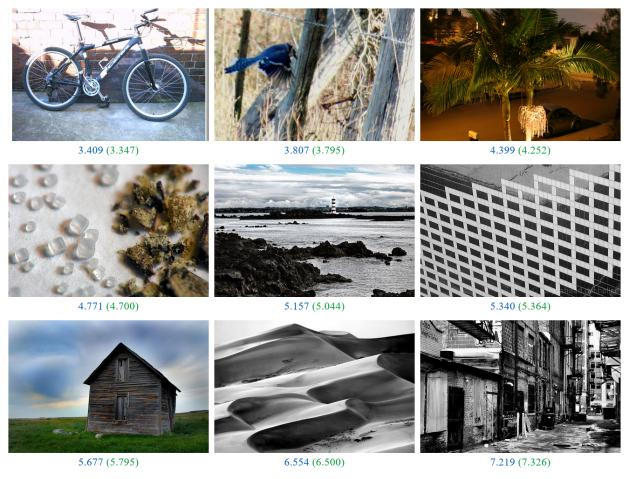
\includegraphics[width=\columnwidth]{fig3_images/ranking_comparison.png}
\caption{Qualitative ranking comparison on nine AVA samples. Images are arranged in a $3\times3$ grid from low to high aesthetic quality by ground-truth and predicted mean scores.}
\label{fig:ranking_comparison}
\end{figure}

\iffalse

\subsubsection{Color/Grayscale figures}
{Figures that are meant to appear in color, or shades of black/gray. Such 
figures may include photographs, illustrations, multicolor graphs, and 
flowcharts.}

\subsubsection{Line Art figures}
{Figures that are composed of only black lines and shapes. These figures 
should have no shades or half-tones of gray, only black and white.}

\subsubsection{Tables}
{Data charts which are typically black and white, but sometimes include 
color.}



\subsection{Multipart figures}
Figures compiled of more than one sub-figure presented side-by-side, or 
stacked. If a multipart figure is made up of multiple figure
types (one part is lineart, and another is grayscale or color) the figure 
should meet the stricter guidelines.

\subsection{File Formats For Graphics}\label{formats}
Format and save your graphics using a suitable graphics processing program 
that will allow you to create the images as PostScript (PS), Encapsulated 
PostScript (.EPS), Tagged Image File Format (.TIFF), Portable Document 
Format (.PDF), Portable Network Graphics (.PNG), or Metapost (.MPS), sizes them, and adjusts 
the resolution settings. When 
submitting your final paper, your graphics should all be submitted 
individually in one of these formats along with the manuscript.

\subsection{Sizing of Graphics}
Most charts, graphs, and tables are one column wide (3.5 inches/88 
millimeters/21 picas) or page wide (7.16 inches/181 millimeters/43 
picas). The maximum depth a graphic can be is 8.5 inches (216 millimeters/54
picas). When choosing the depth of a graphic, please allow space for a 
caption. Figures can be sized between column and page widths if the author 
chooses, however it is recommended that figures are not sized less than 
column width unless when necessary. 

\begin{figure}
\centerline{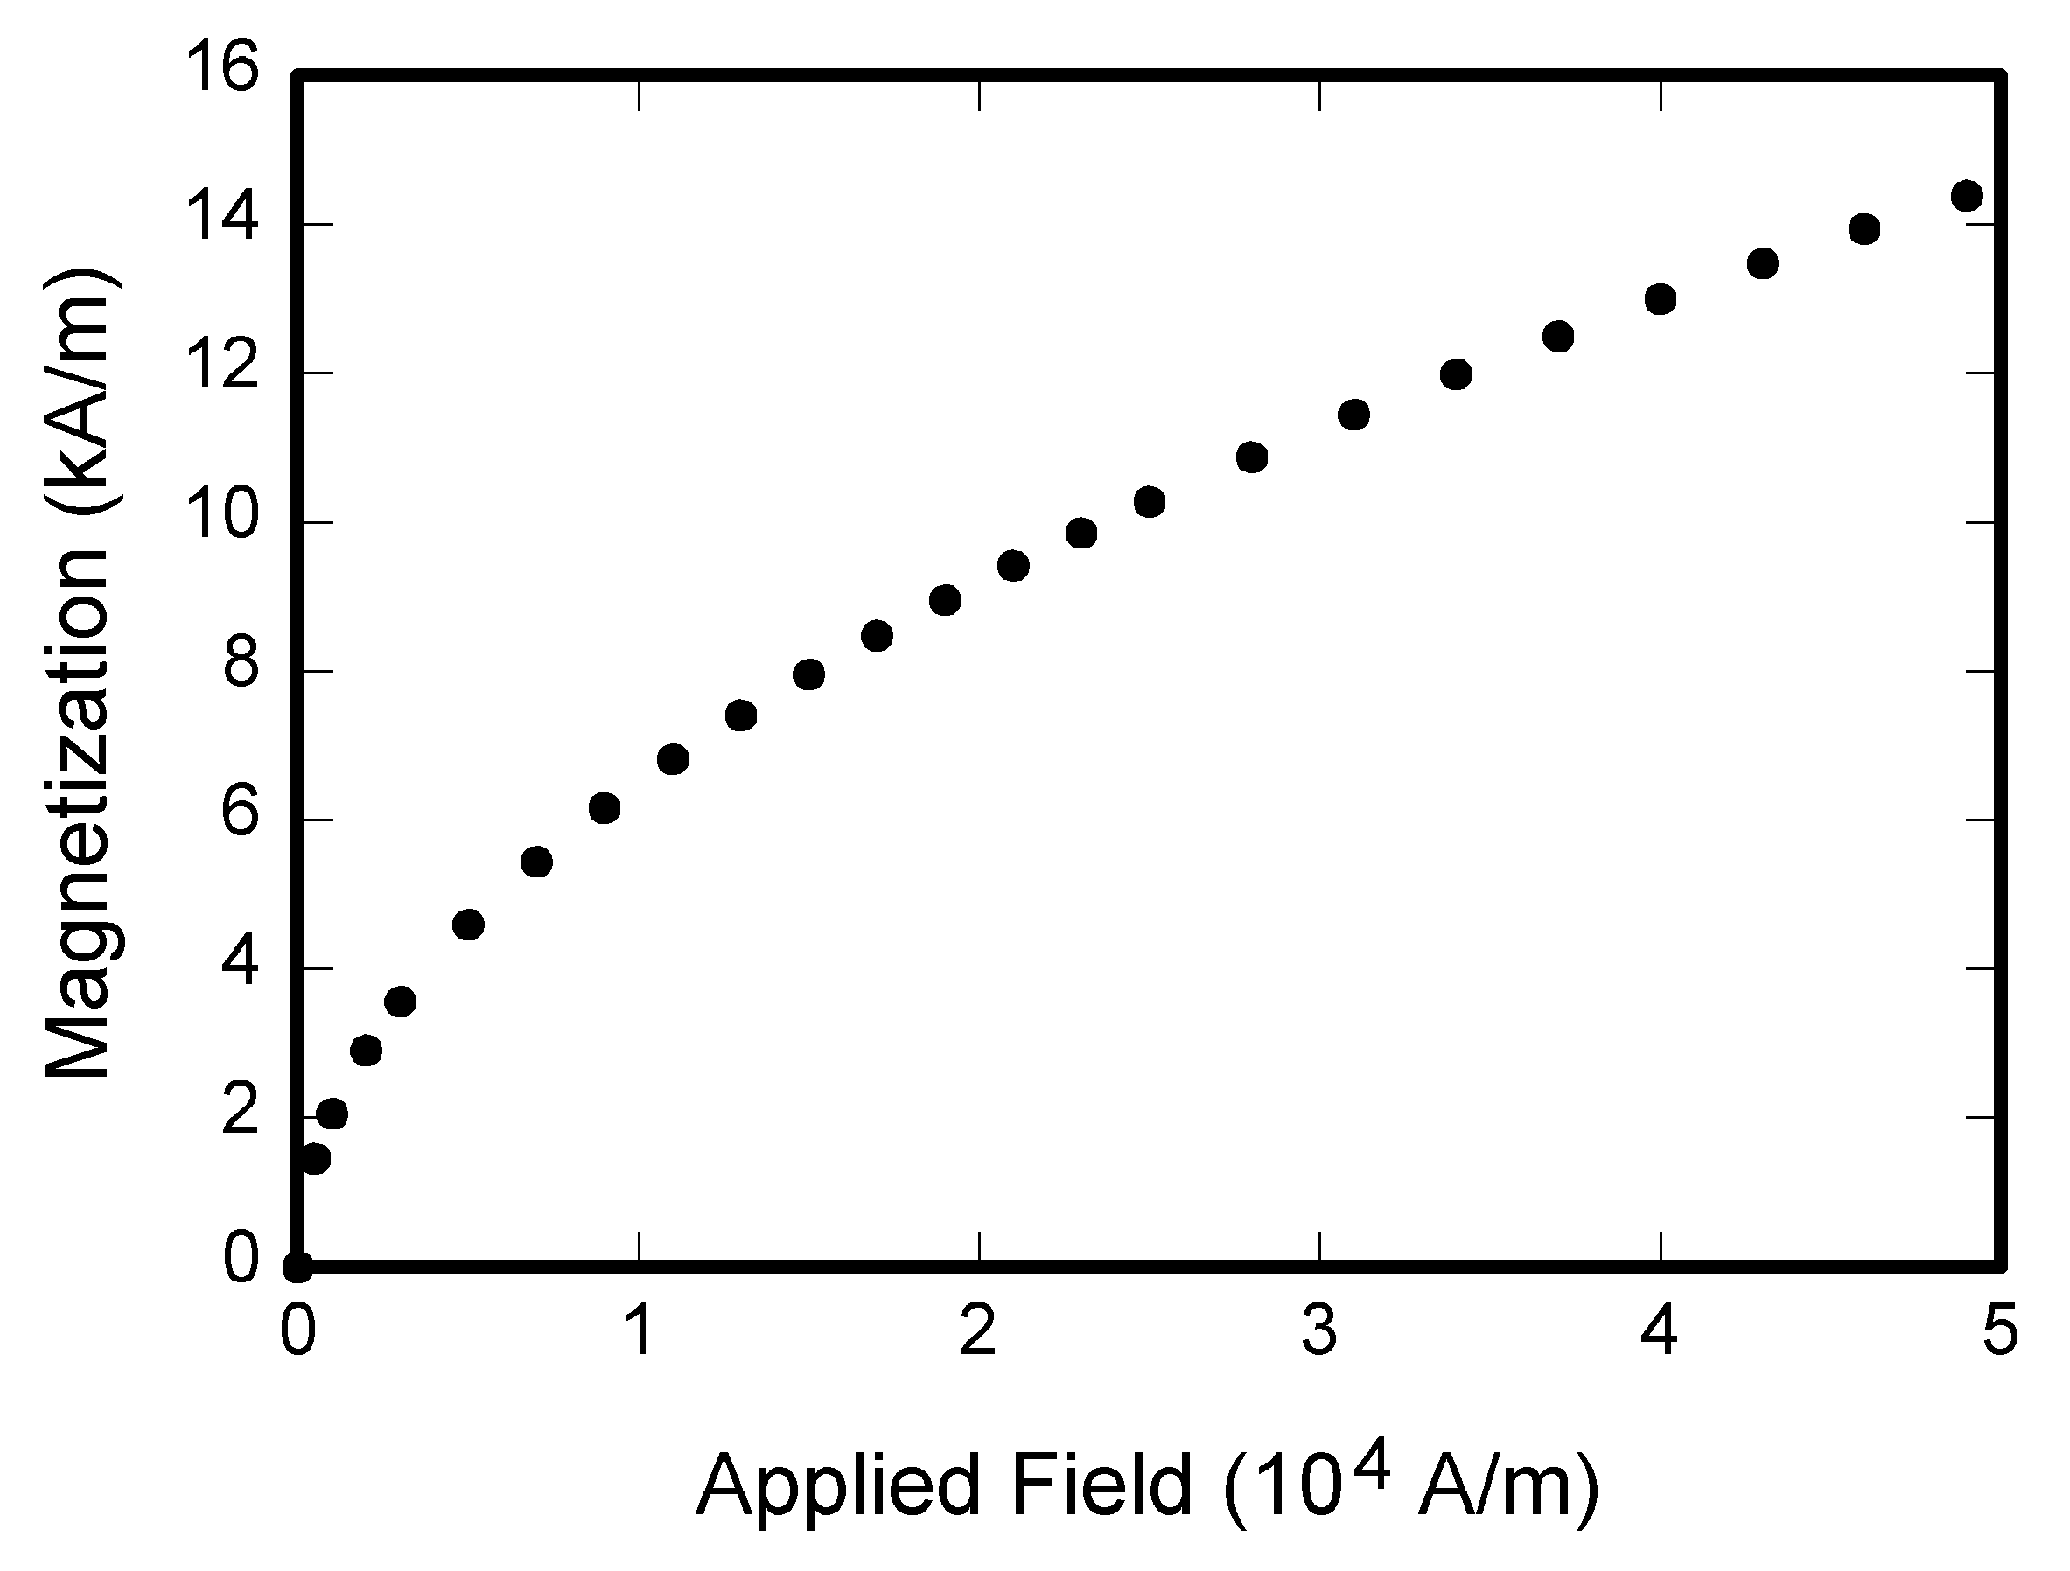
\includegraphics[width=\columnwidth]{fig1.png}}
\caption{Magnetization as a function of applied field. Note that ``Fig.'' is abbreviated. There is a period after the figure number, followed by two spaces. It is good practice to explain the significance of the figure in the caption.}
\end{figure}

\begin{table}
\caption{Units for Magnetic Properties}
\label{table}
\small
\setlength{\tabcolsep}{3pt}
\begin{tabular}{|p{25pt}|p{75pt}|p{110pt}|}
\hline
Symbol& 
Quantity& 
Conversion from Gaussian and \par CGS EMU to SI$^{\mathrm{a}}$ \\
\hline
$\Phi $& 
Magnetic flux& 
1 Mx $\to  10^{-8}$ Wb $= 10^{-8}$ V $\cdot$ s \\
$B$& 
Magnetic flux density, \par magnetic induction& 
1 G $\to  10^{-4}$ T $= 10^{-4}$ Wb/m$^{2}$ \\
$H$& 
Magnetic field strength& 
1 Oe $\to  10^{-3}/(4\pi )$ A/m \\
$m$& 
Magnetic moment& 
1 erg/G $=$ 1 emu \par $\to 10^{-3}$ A $\cdot$ m$^{2} = 10^{-3}$ J/T \\
$M$& 
Magnetization& 
1 erg/(G $\cdot$ cm$^{3}) =$ 1 emu/cm$^{3}$ \par $\to 10^{-3}$ A/m \\
4$\pi M$& 
Magnetization& 
1 G $\to  10^{-3}/(4\pi )$ A/m \\
$\sigma $& 
Specific magnetization& 
1 erg/(G $\cdot$ g) $=$ 1 emu/g $\to $ 1 A $\cdot$ m$^{2}$/kg \\
$j$& 
Magnetic dipole \par moment& 
1 erg/G $=$ 1 emu \par $\to 4\pi \times  10^{-10}$ Wb $\cdot$ m \\
$J$& 
Magnetic polarization& 
1 erg/(G $\cdot$ cm$^{3}) =$ 1 emu/cm$^{3}$ \par $\to 4\pi \times  10^{-4}$ T \\
$\chi , \kappa $& 
Susceptibility& 
1 $\to  4\pi $ \\
$\chi_{\rho }$& 
Mass susceptibility& 
1 cm$^{3}$/g $\to  4\pi \times  10^{-3}$ m$^{3}$/kg \\
$\mu $& 
Permeability& 
1 $\to  4\pi \times  10^{-7}$ H/m \par $= 4\pi \times  10^{-7}$ Wb/(A $\cdot$ m) \\
$\mu_{r}$& 
Relative permeability& 
$\mu \to \mu_{r}$ \\
$w, W$& 
Energy density& 
1 erg/cm$^{3} \to  10^{-1}$ J/m$^{3}$ \\
$N, D$& 
Demagnetizing factor& 
1 $\to  1/(4\pi )$ \\
\hline
\multicolumn{3}{p{251pt}}{Vertical lines are optional in tables. Statements that serve as captions for 
the entire table do not need footnote letters. }\\
\multicolumn{3}{p{251pt}}{$^{\mathrm{a}}$Gaussian units are the same as cg emu for magnetostatics; Mx 
$=$ maxwell, G $=$ gauss, Oe $=$ oersted; Wb $=$ weber, V $=$ volt, s $=$ 
second, T $=$ tesla, m $=$ meter, A $=$ ampere, J $=$ joule, kg $=$ 
kilogram, H $=$ henry.}
\end{tabular}
\label{tab1}
\end{table}


\subsection{Resolution }
The proper resolution of your figures will depend on the type of figure it 
is as defined in the ``Types of Figures'' section. Author photographs, 
color, and grayscale figures should be at least 300dpi. Line art, including 
tables should be a minimum of 600dpi.

\subsection{Vector Art}
In order to preserve the figures' integrity across multiple computer 
platforms, we accept files in the following formats: .EPS/.PDF/.PS. All 
fonts must be embedded or text converted to outlines in order to achieve the 
best-quality results.


\subsection{Accepted Fonts Within Figures}
When preparing your graphics IEEE suggests that you use of one of the 
following Open Type fonts: Times New Roman, Helvetica, Arial, Cambria, and 
Symbol. If you are supplying EPS, PS, or PDF files all fonts must be 
embedded. Some fonts may only be native to your operating system; without 
the fonts embedded, parts of the graphic may be distorted or missing.

A safe option when finalizing your figures is to strip out the fonts before 
you save the files, creating ``outline'' type. This converts fonts to 
artwork what will appear uniformly on any screen.

\subsection{Using Labels Within Figures}

\subsubsection{Figure Axis labels }
Figure axis labels are often a source of confusion. Use words rather than 
symbols. As an example, write the quantity ``Magnetization,'' or 
``Magnetization M,'' not just ``M.'' Put units in parentheses. Do not label 
axes only with units. As in Fig. 1, for example, write ``Magnetization 
(A/m)'' or ``Magnetization (A$\cdot$m$^{-1}$),'' not just ``A/m.'' Do not label axes with a ratio of quantities and 
units. For example, write ``Temperature (K),'' not ``Temperature/K.'' 

Multipliers can be especially confusing. Write ``Magnetization (kA/m)'' or 
``Magnetization (10$^{3}$ A/m).'' Do not write ``Magnetization 
(A/m)$\,\times\,$1000'' because the reader would not know whether the top 
axis label in Fig. 1 meant 16000 A/m or 0.016 A/m. Figure labels should be 
legible, approximately 8 to 10 point type.

\subsubsection{Subfigure Labels in Multipart Figures and Tables}
Multipart figures should be combined and labeled before final submission. 
Labels should appear centered below each subfigure in 8 point Times New 
Roman font in the format of (a) (b) (c). 

\subsection{File Naming}
Figures (line artwork or photographs) should be named starting with the 
first 5 letters of the author's last name. The next characters in the 
filename should be the number that represents the sequential 
location of this image in your article. For example, in author 
``Anderson's'' paper, the first three figures would be named ander1.tif, 
ander2.tif, and ander3.ps.

Tables should contain only the body of the table (not the caption) and 
should be named similarly to figures, except that `.t' is inserted 
in-between the author's name and the table number. For example, author 
Anderson's first three tables would be named ander.t1.tif, ander.t2.ps, 
ander.t3.eps.

\subsection{Referencing a Figure or Table Within Your Paper}
When referencing your figures and tables within your paper, use the 
abbreviation ``Fig.'' even at the beginning of a sentence. Do not abbreviate 
``Table.'' Tables should be numbered with Roman Numerals.

\subsection{Checking Your Figures: The IEEE Graphics Analyzer}
The IEEE Graphics Analyzer enables authors to pre-screen their graphics for 
compliance with IEEE Transactions and Journals standards before submission. 
The online tool, located at
\underline{http://graphicsqc.ieee.org/}, allows authors to 
upload their graphics in order to check that each file is the correct file 
format, resolution, size and colorspace; that no fonts are missing or 
corrupt; that figures are not compiled in layers or have transparency, and 
that they are named according to the IEEE Transactions and Journals naming 
convention. At the end of this automated process, authors are provided with 
a detailed report on each graphic within the web applet, as well as by 
email.

For more information on using the Graphics Analyzer or any other graphics 
related topic, contact the IEEE Graphics Help Desk by e-mail at 
graphics@ieee.org.

\subsection{Submitting Your Graphics}
Because IEEE will do the final formatting of your paper,
you do not need to position figures and tables at the top and bottom of each 
column. In fact, all figures, figure captions, and tables can be placed at 
the end of your paper. In addition to, or even in lieu of submitting figures 
within your final manuscript, figures should be submitted individually, 
separate from the manuscript in one of the file formats listed above in 
Section \ref{formats}. Place figure captions below the figures; place table titles 
above the tables. Please do not include captions as part of the figures, or 
put them in ``text boxes'' linked to the figures. Also, do not place borders 
around the outside of your figures.

\subsection{Color Processing/Printing in IEEE Journals}
All IEEE Transactions, Journals, and Letters allow an author to publish 
color figures on IEEE Xplore\textregistered\ at no charge, and automatically 
convert them to grayscale for print versions. In most journals, figures and 
tables may alternatively be printed in color if an author chooses to do so. 
Please note that this service comes at an extra expense to the author. If 
you intend to have print color graphics, include a note with your final 
paper indicating which figures or tables you would like to be handled that 
way, and stating that you are willing to pay the additional fee.


\fi

\section{Conclusion}

In this letter, we proposed LQ-ICIF, a parameter-efficient multimodal framework for image aesthetic score distribution prediction. By combining learnable query-guided image-comment interaction, hierarchical aggregation, and PARN-based attribute refinement, the proposed method exploits complementary visual, textual, and structured aesthetic features while keeping large pretrained encoders frozen. Experiments and ablation studies on AVA demonstrate the potential of combining user comments and photographic attribute priors for robust and interpretable image aesthetic assessment.

\IEEEtriggeratref{20}
\begin{thebibliography}{40}

\bibitem{datta2006}
R. Datta, D. Joshi, J. Li, and J. Z. Wang, ``Studying aesthetics in photographic images using a computational approach,'' in \emph{Proc. Eur. Conf. Comput. Vis. (ECCV)}, 2006, pp. 288--301.

\bibitem{murray2012ava}
N. Murray, L. Marchesotti, and F. Perronnin, ``AVA: A large-scale database for aesthetic visual analysis,'' in \emph{Proc. IEEE Conf. Comput. Vis. Pattern Recognit. (CVPR)}, 2012, pp. 2408--2415.

\bibitem{talebi2018nima}
H. Talebi and P. Milanfar, ``NIMA: Neural image assessment,'' \emph{IEEE Trans. Image Process.}, vol. 27, no. 8, pp. 3998--4011, Aug. 2018.

\bibitem{kong2016parn}
S. Kong, X. Shen, Z. Lin, R. Mech, and C. Fowlkes, ``Photo aesthetics ranking network with attributes and content adaptation,'' in \emph{Proc. Eur. Conf. Comput. Vis. (ECCV)}, 2016, pp. 662--679.

\bibitem{ke2023vila}
J. Ke, K. Ye, J. Yu, Y. Wu, P. Milanfar, and F. Yang, ``VILA: Learning image aesthetics from user comments with vision-language pretraining,'' arXiv preprint arXiv:2303.14302, 2023.

\bibitem{xiong2024mmlq}
Z. Xiong, Y. Zhang, Z. Shen, P. Ren, and H. Yu, ``Multi-modal learnable queries for image aesthetics assessment,'' arXiv preprint arXiv:2405.01326, 2024.

\bibitem{li2023ammnet}
L. Li, T. Zhu, P. Chen, Y. Yang, Y. Li, and W. Lin, ``Image aesthetics assessment with attribute-assisted multimodal memory network,'' \emph{IEEE Trans. Circuits Syst. Video Technol.}, vol. 33, no. 12, pp. 7413--7424, Dec. 2023.

\bibitem{zhu2023aamnet}
T. Zhu, L. Li, P. Chen, J. Wu, Y. Yang, Y. Li, and Y. Guo, ``Attribute-assisted multimodal network for image aesthetics assessment,'' in \emph{Proc. IEEE Int. Conf. Multimedia Expo (ICME)}, 2023, pp. 2477--2482.

\bibitem{radford2021clip}
A. Radford \emph{et al.}, ``Learning transferable visual models from natural language supervision,'' in \emph{Proc. Int. Conf. Mach. Learn. (ICML)}, 2021, pp. 8748--8763.

\bibitem{devlin2019bert}
J. Devlin, M.-W. Chang, K. Lee, and K. Toutanova, ``BERT: Pre-training of deep bidirectional transformers for language understanding,'' in \emph{Proc. Conf. North Amer. Chapter Assoc. Comput. Linguistics: Hum. Lang. Technol. (NAACL-HLT)}, 2019, pp. 4171--4186.

\bibitem{li2023blip2}
J. Li, D. Li, S. Savarese, and S. Hoi, ``BLIP-2: Bootstrapping language-image pre-training with frozen image encoders and large language models,'' in \emph{Proc. Int. Conf. Mach. Learn. (ICML)}, 2023, pp. 19730--19742.

\bibitem{chang2017pccd}
K. Chang, K.-H. Lu, and C.-S. Chen, ``Aesthetic critiques generation for photos,'' in \emph{Proc. IEEE Int. Conf. Comput. Vis. (ICCV)}, 2017, pp. 3514--3523.

\bibitem{ghosal2019aesthetic}
K. Ghosal, A. Rana, and A. Smolic, ``Aesthetic image captioning from weakly-labelled photographs,'' in \emph{Proc. IEEE/CVF Int. Conf. Comput. Vis. Workshops (ICCVW)}, 2019.

\bibitem{li2025critiques}
L. Li, X. Sheng, P. Chen, J. Wu, and W. Dong, ``Towards explainable image aesthetics assessment with attribute-oriented critiques generation,'' \emph{IEEE Trans. Circuits Syst. Video Technol.}, vol. 35, no. 2, pp. 1464--1477, Feb. 2025.

\bibitem{li2025iaaclip}
Z. Li, X. Yan, X. Wei, and F. Shao, ``IAACLIP: Image aesthetics assessment via CLIP,'' \emph{Electronics}, vol. 14, no. 7, Art. no. 1425, Apr. 2025.

\bibitem{she2021hlagcn}
D. She, Y.-K. Lai, G. Yi, and K. Xu, ``Hierarchical layout-aware graph convolutional network for unified aesthetics assessment,'' in \emph{Proc. IEEE/CVF Conf. Comput. Vis. Pattern Recognit. (CVPR)}, 2021, pp. 8475--8484.

\bibitem{ke2021musiq}
J. Ke, Q. Wang, Y. Wang, P. Milanfar, and F. Yang, ``MUSIQ: Multi-scale image quality transformer,'' in \emph{Proc. IEEE/CVF Int. Conf. Comput. Vis. (ICCV)}, 2021, pp. 5148--5157.

\bibitem{he2022tanet}
S. He, Y. Zhang, R. Xie, D. Jiang, and A. Ming, ``Rethinking image aesthetics assessment: Models, datasets and benchmarks,'' in \emph{Proc. Int. Joint Conf. Artif. Intell. (IJCAI)}, 2022, pp. 942--948.

\bibitem{xiong2023iaalq}
Z. Xiong, Y. Zhang, Z. Shen, P. Ren, and H. Yu, ``Image aesthetics assessment via learnable queries,'' arXiv preprint arXiv:2309.02861, 2023.

\bibitem{gao2024aesmamba}
F. Gao, Y. Lin, J. Shi, M. Qiao, and N. Wang, ``AesMamba: Universal image aesthetic assessment with state space models,'' in \emph{Proc. ACM Int. Conf. Multimedia (MM)}, 2024, pp. 7444--7454.

\bibitem{shi2024milnet}
T. Shi, C. Chen, Z. Wu, A. Hao, and Y. Fang, ``Improving image aesthetic assessment via multiple image joint learning,'' \emph{ACM Trans. Multimedia Comput. Commun. Appl.}, vol. 20, no. 11, Art. no. 355, Nov. 2024.

\bibitem{hou2025tcdg}
J. Hou, W. Lin, Y. Fang, H. Wu, C. Chen, L. Liao, and W. Liu, ``Toward transparent deep image aesthetics assessment with tag-based content descriptors,'' \emph{IEEE Trans. Image Process.}, vol. 34, pp. 3070--3084, 2025.

\bibitem{zhang2019gpfcnn}
X. Zhang, X. Gao, W. Lu, and L. He, ``A gated peripheral-foveal convolutional neural network for unified image aesthetic prediction,'' \emph{IEEE Trans. Multimedia}, vol. 21, no. 11, pp. 2815--2826, Nov. 2019.

\bibitem{zhang2021mscan}
X. Zhang, X. Gao, L. He, and W. Lu, ``MSCAN: Multimodal self-and-collaborative attention network for image aesthetic prediction tasks,'' \emph{Neurocomputing}, vol. 430, pp. 14--23, Mar. 2021.

\bibitem{behrad2025charm}
F. Behrad, T. Tuytelaars, and J. Wagemans, ``Charm: The missing piece in ViT fine-tuning for image aesthetic assessment,'' in \emph{Proc. IEEE/CVF Conf. Comput. Vis. Pattern Recognit. (CVPR)}, 2025, pp. 7815--7824.

\bibitem{deng2017survey}
Y. Deng, C. C. Loy, and X. Tang, ``Image aesthetic assessment: An experimental survey,'' \emph{IEEE Signal Process. Mag.}, vol. 34, no. 4, pp. 80--106, Jul. 2017.

\bibitem{dhar2011high}
S. Dhar, V. Ordonez, and T. L. Berg, ``High level describable attributes for predicting aesthetics and interestingness,'' in \emph{Proc. IEEE Conf. Comput. Vis. Pattern Recognit. (CVPR)}, 2011, pp. 1657--1664.

\bibitem{marchesotti2011generic}
L. Marchesotti, F. Perronnin, D. Larlus, and G. Csurka, ``Assessing the aesthetic quality of photographs using generic image descriptors,'' in \emph{Proc. IEEE Int. Conf. Comput. Vis. (ICCV)}, 2011, pp. 1784--1791.

\bibitem{mai2016composition}
L. Mai, H. Jin, and F. Liu, ``Composition-preserving deep photo aesthetics assessment,'' in \emph{Proc. IEEE Conf. Comput. Vis. Pattern Recognit. (CVPR)}, 2016, pp. 497--506.

\bibitem{ma2017alamp}
S. Ma, J. Liu, and C. W. Chen, ``A-Lamp: Adaptive layout-aware multi-patch deep convolutional neural network for photo aesthetic assessment,'' in \emph{Proc. IEEE Conf. Comput. Vis. Pattern Recognit. (CVPR)}, 2017, pp. 4535--4544.

\bibitem{wang2016bdn}
Z. Wang, S. Chang, F. Dolcos, D. Beck, D. Liu, and T. S. Huang, ``Brain-inspired deep networks for image aesthetics assessment,'' arXiv preprint arXiv:1601.04155, 2016.

\bibitem{ren2017personalized}
J. Ren, X. Shen, Z. Lin, R. Mech, and D. J. Foran, ``Personalized image aesthetics,'' in \emph{Proc. IEEE Int. Conf. Comput. Vis. (ICCV)}, 2017, pp. 638--647.

\bibitem{celona2022composition}
L. Celona, M. Leonardi, P. Napoletano, and A. Rozza, ``Composition and style attributes guided image aesthetic assessment,'' \emph{IEEE Trans. Image Process.}, vol. 31, pp. 5009--5024, 2022.

\bibitem{anwar2022comparative}
A. Anwar, S. Kanwal, M. Tahir, M. Saqib, M. Uzair, M. K. I. Rahmani, and H. Ullah, ``Image aesthetic assessment: A comparative study of hand-crafted and deep learning models,'' \emph{IEEE Access}, vol. 10, pp. 101770--101789, 2022.

\bibitem{vaswani2017attention}
A. Vaswani \emph{et al.}, ``Attention is all you need,'' in \emph{Proc. Adv. Neural Inf. Process. Syst. (NeurIPS)}, 2017, pp. 5998--6008.

\bibitem{dosovitskiy2021vit}
A. Dosovitskiy \emph{et al.}, ``An image is worth 16x16 words: Transformers for image recognition at scale,'' in \emph{Proc. Int. Conf. Learn. Represent. (ICLR)}, 2021.

\bibitem{li2022blip}
J. Li, D. Li, C. Xiong, and S. Hoi, ``BLIP: Bootstrapping language-image pre-training for unified vision-language understanding and generation,'' in \emph{Proc. Int. Conf. Mach. Learn. (ICML)}, 2022, pp. 12888--12900.

\bibitem{zhou2022coop}
K. Zhou, J. Yang, C. C. Loy, and Z. Liu, ``Learning to prompt for vision-language models,'' \emph{Int. J. Comput. Vis.}, vol. 130, no. 9, pp. 2337--2348, Sep. 2022.

\bibitem{jia2022vpt}
M. Jia, L. Tang, B.-C. Chen, C. Cardie, S. Belongie, B. Hariharan, and S.-N. Lim, ``Visual prompt tuning,'' in \emph{Proc. Eur. Conf. Comput. Vis. (ECCV)}, 2022, pp. 709--727.

\bibitem{hu2022lora}
E. J. Hu, Y. Shen, P. Wallis, Z. Allen-Zhu, Y. Li, S. Wang, L. Wang, and W. Chen, ``LoRA: Low-rank adaptation of large language models,'' in \emph{Proc. Int. Conf. Learn. Represent. (ICLR)}, 2022.

\end{thebibliography}

\iffalse
\section*{Acknowledgment}

The preferred spelling of the word ``acknowledgment'' in American English is without an ``e'' after the ``g.'' Use the singular heading even if you have many acknowledgments. Avoid expressions such as ``One of us (S.B.A.) would like to thank . . . .'' Instead, write “F. A. Author thanks ... .” In most cases, sponsor and financial support acknowledgments are placed in the unnumbered footnote on the first page, not here.

\section*{References and Footnotes}

\subsection{References}

References need not be cited in text. When they are, they appear on the line, in square brackets, inside the punctuation.  Multiple references are each numbered with separate brackets. When citing a section in a book, please give the relevant page numbers. In text, refer simply to the reference number. Do not use ``Ref.'' or ``reference'' except at the beginning of a sentence: ``Reference [3] shows . . . .'' Please do not use automatic endnotes in {\em Word}, rather, type the reference list at the end of the paper using the ``References'' style.

Reference numbers are set flush left and form a column of their own, hanging out beyond the body of the reference. The reference numbers are on the line, enclosed in square brackets. In all references, the given name of the author or editor is abbreviated to the initial only and precedes the last name. Use them all; use {\em et al.} only if names are not given. Use commas around Jr., Sr., and III in names. Abbreviate conference titles.  When citing IEEE transactions, provide the issue number, page range, volume number, year, and/or month if available. When referencing a patent, provide the day and the month of issue, or application. References may not include all information; please obtain and include relevant information. Do not combine references. There must be only one reference with each number. If there is a URL included with the print reference, it can be included at the end of the reference.

Other than books, capitalize only the first word in a paper title, except for proper nouns and element symbols. For papers published in translation journals, please give the English citation first, followed by the original foreign-language citation. See the end of this document for formats and examples of common references. For a complete discussion of references and their formats, see the IEEE style manual at www.ieee.org/authortools.

\subsection{Footnotes}

Number footnotes separately in superscripts (Insert $\mid$ Footnote).\footnote{It is recommended that footnotes be avoided (except for the unnumbered footnote with the receipt date on the first page). Instead, try to integrate the footnote information into the text.}  Place the actual footnote at the bottom of the column in which it is cited; do not put footnotes in the reference list (endnotes). Use letters for table footnotes (see Table I). 


\section*{References}

\subsection*{Basic format for books:}

J. K. Author, ``Title of chapter in the book,'' in {\em Title of His Published Book}, xth ed. City of Publisher, (only U.S. State), Country: Abbrev. of Publisher, year, ch. x, sec. x, pp. xxx--xxx.

\subsection*{Examples:}
\def\refname{}
\begin{thebibliography}{34}

\bibitem{}G. O. Young, ``Synthetic structure of industrial plastics,'' in {\em Plastics}, 2nd ed., vol. 3, J. Peters, Ed. New York, NY, USA: McGraw-Hill, 1964, pp. 15--64.

\bibitem{}W.-K. Chen, {\it Linear Networks and Systems}. Belmont, CA, USA: Wadsworth, 1993, pp. 123--135.

\end{thebibliography}

\subsection*{Basic format for periodicals:}

J. K. Author, ``Name of paper,'' Abbrev. Title of Periodical, vol. x,   no. x, pp. xxx--xxx, Abbrev. Month, year, DOI. 10.1109.XXX.123--456.

\subsection*{Examples:}

\begin{thebibliography}{34}
\setcounter{enumiv}{2}

\bibitem{}J. U. Duncombe, ``Infrared navigation Part I: An assessment of feasibility,'' {\em IEEE Trans. Electron Devices}, vol. ED-11, no. 1, pp. 34--39, Jan. 1959,10.1109/TED.2016.2628402.

\bibitem{}E. P. Wigner, ``Theory of traveling-wave optical laser,''
{\em Phys. Rev.},  vol. 134, pp. A635--A646, Dec. 1965.

\bibitem{}E. H. Miller, ``A note on reflector arrays,'' {\em IEEE Trans. Antennas Propagat.}, to be published.
\end{thebibliography}


\subsection*{Basic format for reports:}

J. K. Author, ``Title of report,'' Abbrev. Name of Co., City of Co., Abbrev. State, Country, Rep. xxx, year.

\subsection*{Examples:}
\begin{thebibliography}{34}
\setcounter{enumiv}{5}

\bibitem{} E. E. Reber, R. L. Michell, and C. J. Carter, ``Oxygen absorption in the earth’s atmosphere,'' Aerospace Corp., Los Angeles, CA, USA, Tech. Rep. TR-0200 (4230-46)-3, Nov. 1988.

\bibitem{} J. H. Davis and J. R. Cogdell, ``Calibration program for the 16-foot antenna,'' Elect. Eng. Res. Lab., Univ. Texas, Austin, TX, USA, Tech. Memo. NGL-006-69-3, Nov. 15, 1987.
\end{thebibliography}

\subsection*{Basic format for handbooks:}

{\em Name of Manual/Handbook}, x ed., Abbrev. Name of Co., City of Co., Abbrev. State, Country, year, pp. xxx--xxx.

\subsection*{Examples:}

\begin{thebibliography}{34}
\setcounter{enumiv}{7}

\bibitem{} {\em Transmission Systems for Communications}, 3rd ed., Western Electric Co., Winston-Salem, NC, USA, 1985, pp. 44--60.

\bibitem{} {\em Motorola Semiconductor Data Manual}, Motorola Semiconductor Products Inc., Phoenix, AZ, USA, 1989.
\end{thebibliography}

\subsection*{Basic format for books (when available online):}

J. K. Author, ``Title of chapter in the book,'' in {\em Title of Published Book}, xth ed. City of Publisher, State, Country: Abbrev. of Publisher, year, ch. x, sec. x, pp. xxx xxx. [Online]. Available: http://www.web.com 

\subsection*{Examples:}

\begin{thebibliography}{34}
\setcounter{enumiv}{9}

\bibitem{}G. O. Young, ``Synthetic structure of industrial plastics,'' in Plastics, vol. 3, Polymers of Hexadromicon, J. Peters, Ed., 2nd ed. New York, NY, USA: McGraw-Hill, 1964, pp. 15--64. [Online]. Available: http://www.bookref.com. 

\bibitem{} {\em The Founders Constitution}, Philip B. Kurland and Ralph Lerner, eds., Chicago, IL, USA: Univ. Chicago Press, 1987. [Online]. Available: http://press-pubs.uchicago.edu/founders/

\bibitem{} The Terahertz Wave eBook. ZOmega Terahertz Corp., 2014. [Online]. Available: http://dl.z-thz.com/eBook/zomega\_ebook\_pdf\_1206\_sr.pdf. Accessed on: May 19, 2014. 

\bibitem{} Philip B. Kurland and Ralph Lerner, eds., {\em The Founders Constitution}. Chicago, IL, USA: Univ. of Chicago Press, 1987, Accessed on: Feb. 28, 2010, [Online] Available: http://press-pubs.uchicago.edu/founders/ 
\end{thebibliography}

\subsection*{Basic format for journals (when available online):}

J. K. Author, ``Name of paper,'' {\em Abbrev. Title of Periodical}, vol. x, no. x, pp. xxx--xxx, Abbrev. Month, year. Accessed on: Month, Day, year, doi: 10.1109.XXX.123456, [Online].

\subsection*{Examples:}

\begin{thebibliography}{34}
\setcounter{enumiv}{13}

\bibitem{}J. S. Turner, ``New directions in communications,'' {\em IEEE J. Sel. Areas Commun.}, vol. 13, no. 1, pp. 11--23, Jan. 1995. 

\bibitem{} W. P. Risk, G. S. Kino, and H. J. Shaw, ``Fiber-optic frequency shifter using a surface acoustic wave incident at an oblique angle,'' {\em Opt. Lett.}, vol. 11, no. 2, pp. 115--117, Feb. 1986.

\bibitem{} P. Kopyt {\em et al.}, ``Electric properties of graphene-based conductive layers from DC up to terahertz range,'' {\em IEEE THz Sci. Technol.}, to be published. doi: 10.1109/TTHZ.2016.2544142.
\end{thebibliography}

\subsection*{Basic format for papers presented at conferences (when available online):}

J.K. Author. (year, month). Title. presented at abbrev. conference title. [Type of Medium]. Available: site/path/file

\subsection*{Example:}

\begin{thebibliography}{34}
\setcounter{enumiv}{16}

\bibitem{}PROCESS Corporation, Boston, MA, USA. Intranets: Internet technologies deployed behind the firewall for corporate productivity. Presented at INET96 Annual Meeting. [Online]. Available: http://home.process.com/Intranets/wp2.htp
\end{thebibliography}

\subsection*{Basic format for reports  and  handbooks (when available online):}
  
J. K. Author. ``Title of report,'' Company. City, State, Country. Rep. no., (optional: vol./issue), Date. [Online] Available: site/path/file 

\subsection*{Examples:}

\begin{thebibliography}{34}
\setcounter{enumiv}{17}

\bibitem{}R. J. Hijmans and J. van Etten, ``Raster: Geographic analysis and modeling with raster data,'' R Package Version 2.0-12, Jan. 12, 2012. [Online]. Available: http://CRAN.R-project.org/package=raster 

\bibitem{}Teralyzer. Lytera UG, Kirchhain, Germany [Online]. Available: http://www.lytera.de/Terahertz\_THz\_Spectroscopy.php?id=home, Accessed on: Jun. 5, 2014.
\end{thebibliography}

\subsection*{Basic format for computer programs and electronic documents (when available online):}

Legislative body. Number of Congress, Session. (year, month day). {\em Number of bill or resolution, Title}. [Type of medium]. Available: site/path/file
{\em NOTE:} ISO recommends that capitalization follow the accepted practice for the language or script in which the information is given.

\subsection*{Example:}

\begin{thebibliography}{34}
\setcounter{enumiv}{19}

\bibitem{}U. S. House. 102nd Congress, 1st Session. (1991, Jan. 11). {\em H. Con. Res. 1, Sense of the Congress on Approval of Military Action}. [Online]. Available: LEXIS Library: GENFED File: BILLS 
\end{thebibliography}

\subsection*{Basic format for patents (when available online):}

Name of the invention, by inventor’s name. (year, month day). Patent Number [Type of medium]. Available:site/path/file

\subsection*{Example:}

\begin{thebibliography}{34}
\setcounter{enumiv}{20}

\bibitem{}Musical tooth brush with mirror, by L. M. R. Brooks. (1992, May 19). Patent D 326 189
[Online]. Available: NEXIS Library: LEXPAT File:   DES 

\end{thebibliography}

\subsection*{Basic format for conference proceedings (published):}

J. K. Author, ``Title of paper,'' in {\em Abbreviated Name of Conf.}, City of Conf., Abbrev. State (if given), Country, year, pp. xxx--xxx.

\subsection*{Example:}

\begin{thebibliography}{34}
\setcounter{enumiv}{21}

\bibitem{}D. B. Payne and J. R. Stern, ``Wavelength-switched passively coupled single-mode optical network,'' in {\em Proc. IOOC-ECOC}, Boston, MA, USA, 1985,
pp. 585--590.

\end{thebibliography}

\subsection*{Example for papers presented at conferences (unpublished):}

\begin{thebibliography}{34}
\setcounter{enumiv}{22}

\bibitem{}D. E behard and E. Voges, ``Digital single sideband detection for inter ferometric sensors,'' presented at the {\em 2nd Int. Conf. Optical Fiber Sensors}, Stuttgart, Germany, Jan. 2--5, 1984.
\end{thebibliography}

\subsection*{Basic formatfor patents:}

J. K. Author, ``Title of patent,'' U. S. Patent x xxx xxx, Abbrev. Month, day, year.

\subsection*{Example:}

\begin{thebibliography}{34}
\setcounter{enumiv}{23}

\bibitem{}G. Brandli and M. Dick, ``Alternating current fed power supply,'' U. S. Patent 4 084 217, Nov. 4, 1978.
\end{thebibliography}

\subsection*{Basic format for theses (M.S.) and dissertations (Ph.D.):}

a) J. K. Author, ``Title of thesis,'' M. S. thesis, Abbrev. Dept., Abbrev. Univ., City of Univ., Abbrev. State, year.

b) J. K. Author, ``Title of dissertation,'' Ph.D. dissertation, Abbrev. Dept., Abbrev. Univ., City of Univ., Abbrev. State, year.

\subsection*{Examples:}

\begin{thebibliography}{34}
\setcounter{enumiv}{24}

\bibitem{}J. O. Williams, ``Narrow-band analyzer,'' Ph.D. dissertation, Dept. Elect. Eng., Harvard Univ., Cambridge, MA, USA, 1993.

\bibitem{}N. Kawasaki, ``Parametric study of thermal and chemical nonequilibrium nozzle flow,'' M.S. thesis, Dept. Electron. Eng., Osaka Univ., Osaka, Japan, 1993.
\end{thebibliography}

\subsection*{Basic format for the most common types of unpublished references:}

a) J. K. Author, private communication, Abbrev. Month, year.

b) J. K. Author, ``Title of paper,'' unpublished.

c) J. K. Author, ``Title of paper,'' to be published.

\subsection*{Examples:}

\begin{thebibliography}{34}
\setcounter{enumiv}{26}

\bibitem{}A. Harrison, private communication, May 1995.

\bibitem{}B. Smith, ``An approach to graphs of linear forms,'' unpublished.

\bibitem{}A. Brahms, ``Representation error for real numbers in binary computer arithmetic,'' IEEE Computer Group Repository, Paper R-67-85.
\end{thebibliography}

\subsection*{Basic formats for standards:}

a) {\em Title of Standard}, Standard number, date.

b) {\em Title of Standard}, Standard number, Corporate author, location, date.

\subsection*{Examples:}

\begin{thebibliography}{34}
\setcounter{enumiv}{29}


\bibitem{}IEEE Criteria for Class IE Electric Systems, IEEE Standard 308, 1969.

\bibitem{} Letter Symbols for Quantities, ANSI Standard Y10.5-1968.
\end{thebibliography}

\subsection*{Article number in reference examples:}

\begin{thebibliography}{34}
\setcounter{enumiv}{31}

\bibitem{}R. Fardel, M. Nagel, F. Nuesch, T. Lippert, and A. Wokaun, ``Fabrication of organic light emitting diode pixels by laser-assisted forward transfer,'' {\em Appl. Phys. Lett.}, vol. 91, no. 6, Aug. 2007, Art. no. 061103. 

\bibitem{} J. Zhang and N. Tansu, ``Optical gain and laser characteristics of InGaN quantum wells on ternary InGaN substrates,'' {\em IEEE Photon.} J., vol. 5, no. 2, Apr. 2013, Art. no. 2600111
\end{thebibliography}

\subsection*{Example when using et al.:}

\begin{thebibliography}{34}
\setcounter{enumiv}{33}

\bibitem{}S. Azodolmolky {\em et al.}, Experimental demonstration of an impairment aware network planning and operation tool for transparent/translucent optical networks,'' {\em J. Lightw. Technol.}, vol. 29, no. 4, pp. 439--448, Sep. 2011.
\end{thebibliography}

\fi

\end{document}
